\chapter{Redes neuronales: Deep Learning}
\lsection{Redes neuronales}
\subsection {Historia de las redes neuronales}
TODO: Agrupar los items por fechas amplias: 50s, 60s...\\
TODO: mencionar a Hinton-Sejnowski\\
Las redes neuronales, como su nombre indica, pretenden imitar la forma de funcionamiento de las neuronas que forman el cerebro humano.
\begin{itemize}
\item Entre los pioneros en el modelado de neuronas se encuentra Warren McCulloch y Walter Pitts, investigadores que propusieron un modelo matemático.
\item En 1949, Hebb definió dos conceptos muy importantes:
\begin{itemize}
\item El proceso de aprendizaje se localiza principalmente en la sinapsis o conexión entre neuronas.
\item La información se representa en el cerebro mediante un conjunto de neuronas activas o inactivas.
\end{itemize}
Estas dos reglas se sintetizan en la regla de aprendizaje de Hebb, que sigue siendo usada en algunos modelos actuales. Esta regla nos dice que los cambios en los pesos de la sinapsis se basan en la interacción entre las neuronas pre y post sintacticas, y el numero de veces que se activan de manera simultanea.
\item En 1956, en la ciudad de Dartmouth, se llevó a cabo la primera conferencia sobre Inteligencia Artificial donde se discutió sobre la capacidad de las maquinas para simular el aprendizaje humano.
\item En 1959, Widrow escribió la Teoría sobre la adaptación neuronal, y desarrolló los Algoritmos Adaline (Adaptative Linear Neuron) y Madaline (Multiple Adaline). Con ellos, se consiguió llevar a cabo la primera aplicación de redes neuronales para solventar problemas reales: un filtro para eliminar ecos en las lineas telefonicas.
\item En 1962 Rosemblatt desarrolló el concepto de perceptrón. Esto dio lugar a la regla de aprendizaje Delta, que permitía emplear señales continuas de entrada y de salida.
\item En 1984, Kohonen desarrolló una familia de redes de memoria asociativa y mapas auto-organizativos, actualmente llamadas redes de Kohonen.
\item Anderson desarrolló una red denominada Brain-State-in-a-Box, la cual trunca la salida lineal para que no se vuelva demasiado grande en las iteraciones de la red.
\item Grossberg y Carpenter desarrollaron las redes autoorganizativas de categorías ART (Teoria de la Resonancia Adaptativa)
\item Mediante las redes de Hopfield, se demostró que las redes asociativas pueden aprender por analogía a la autoorganización de los sistemas físicos.
\item Neocognitrón: Kinihiko Fukushima desarrolló una familia de redes para el reconocimiento de caracteres.
\item Mediante las máquinas de Boltzman se desarrolló la regla de aprendizaje basada en funciones de densidad de probabilidad.
\end{itemize}

\begin{figure}[htp]
\centering
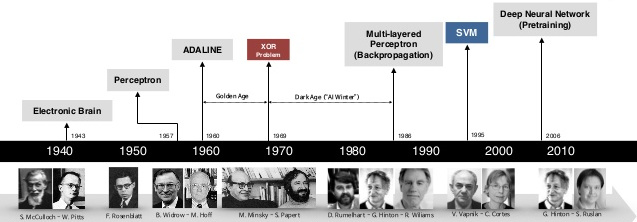
\includegraphics[scale=0.60]{images/history.jpg}
\caption{Historia de las redes neuronales}
\end{figure}

\subsection {La neurona biologica} \mbox{}\\
El cerebro, visto a un alto nivel y simplificando enormemente su estructura, podríamos decir que es un conjunto de millones y millones de células, llamadas neuronas, interconectadas entre ellas mediante sinapsis. La sinapsis se lleva a cabo en la zona donde 2 neuronas se conectan, y las partes de la célula que se encargan de realizarla son las dendritas y las ramificaciones del axón.
\begin{figure}[htp]
\centering
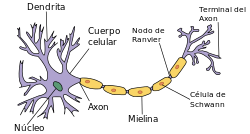
\includegraphics[scale=1]{images/neurona.png}
\caption{Estructura de una neurona}
\end{figure}\\
Cada neurona desarrolla impulsos eléctricos que se trasmiten a lo largo de esta mediante su axón. Este, al final se ramifica en ramificaciones axionales, que conectan con otras neuronas mediante sus dentritras.\\
El conjunto de elementos que hay entre la ramificación axional y la dendrita forman la sinapsis, que regula la transmisión del impulso eléctrico mediante unos elementos químicos llamados neurotransmisores.
\begin{figure}[htp]
\centering
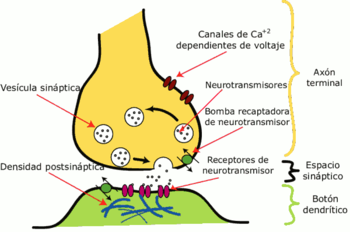
\includegraphics[scale=0.70]{images/sinapsis.png}
\caption{Sinapsis}
\end{figure}\\
Los neurotransmisores liberados en la sinapsis pueden tener un efecto negativo o positivo sobre la transmisión del impulso eléctrico en la neurona que los recibe en sus dendritas. Esta neurona recibe varias señales de las distintas sinapsis, y las combina consiguiendo un cierto nivel de estimulación. En función de este nivel de activación, la neurona emite señales eléctricas mediante impulsos, con una intensidad determinada y con una frecuencia llamada tasa de disparo.\\
En resumen, si consideramos que la información del cerebro está codificada en impulsos eléctricos que se transmiten entre neuronas, y que los impulsos se ven modificados básicamente en la sinapsis, podemos intuir que la codificación del aprendizaje estará en la sinapsis y en la forma en la que las neuronas dejan pasar o inhiben las señales segregando neurotransmisores.

\subsection {La neurona artificial} \mbox{}
Las neuronas artificiales son modelos que tratan de simular el comportamiento de las neuronas biológicas. Cada neurona se representa como una unidad de proceso que forma parte de una entidad mayor, la red neuronal.
\begin{figure}[htp]
\centering
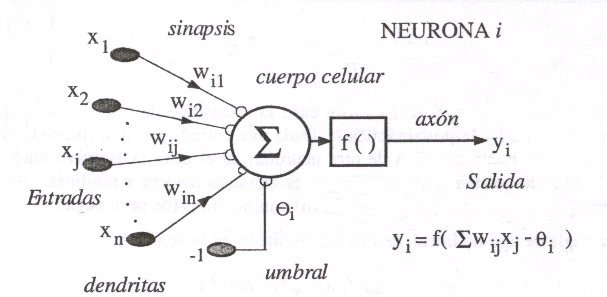
\includegraphics[scale=1]{images/neuronaartificial.jpg}
\caption{Esquema de una neurona artificial}
\end{figure}\\
Como podemos intuir observando la imagen anterior, la neurona artificial se comporta en cierto modo como una biológica, pero de forma simplificada:
\begin{itemize}
\item Entradas (${x_{1}, x_{2}}$): estos valores pueden ser enteros, reales o binarios y equivaldrían a los impulsos que envían otras neuronas a través de sus dendritas.
\item Pesos (${w_{1}, w_{2}}$): equivaldrían a los mecanismos de sinapsis para transmitir el impulso.
\item De este modo, el producto de los valores ${x_{i} , w_{i}}$ equivaldría a las señales químicas inhibidoras y excitadoras que se dan en la neurona. Estos valores son la entrada de la función de activación, que convierte todo el conjunto de valores en uno solo llamado potencial. La función de ponderación suele ser la suma ponderada de las entradas y los pesos sinápticos.
\item La salida de función de ponderación llega a la función de activación que transforma este valor en otro en el dominio que trabajen las salidas de las neuronas. Suele ser una función no lineal como la función paso o la función sigmoide, aunque también se usa funciones lineales.
\item El valor de salida cumpliría la función de la tasa de disparo en las neuronas biológicas.
\end{itemize}
En resumen, podemos establecer las siguientes analogías:
\begin{itemize}
\item Neuronas biológicas $\Longleftrightarrow$ Neuronas Artificiales.
\item Conexiones sinápticas $\Longleftrightarrow$ Conexiones ponderadas.
\item Efectividad de las sinapsis$\Longleftrightarrow$ Peso de las conexiones.
\item Efecto excitador o inhibidor de una conexión $\Longleftrightarrow$ Signo del peso de una
conexión.
\item Activación $\rightarrow$ Tasa de disparo $\Longleftrightarrow$ Función de activación $\rightarrow$ Salida
\end{itemize}

\subsection {Funciones de las neuronas artificiales}
\subsubsection {Función de red o propagación}
TODO: No entiendo bien lo que quieres decir\\
Esta función se encarga de transformar las diferentes entradas que provienen de la sinapsis, en el potencial de la neurona. Normalmente, las neuronas han de tratar simultáneamente con varios valores de entrada, y han de hacerlo como si se tratase de uno solo. Esta función viene a resolver el problema de combinar las entradas simples (${x_{1},x_{2},x_{3}...}$) en una sola entrada global. Podría describirme mediante la siguiente ecuación:
\begin{equation}
input = (x_{1}:w_{1})*(x_{2}:w_{2})*...*(x_{n}:w_{n})
\end{equation}
siendo ":" el operador apropiado (por ejemplo: máximo, sumatorio, producto...), "n" el numero de entradas y w el peso de las conexiones. Multiplicando las entradas por los pesos, se permite que un valo muy grande de entrada pueda tener una influencia pequeña, si sus pesos son pequeños.
\subsubsection {Función de activación}
La función de activación combina el potencial que nos proporciona la función de propagación con el estado actual de la neurona, para conseguir el estado futuro de esta (activada/desactivada). Esta función es normalmente creciente y monótona. Las funciones mas comunes son:
\begin{itemize}
\item Identidad: es una función de activación muy simple que siempre devuelve como salida su valor de entrada. Su rango es va de menos infinito a infinito, es monótona y derivativamente monótona.
\begin{equation}
f(x) = x
\end{equation}
\begin{figure}[htp]
\centering
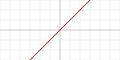
\includegraphics[scale=1]{images/Activation_identity.png}
\caption{Funcion de activación identidad}
\end{figure}
\item Escalón binario: Es la más usada por redes neuronales binarias ya que no es lineal, y es bastante sencilla. El Perceptrón y Hopfield son algunos ejemplos de redes que usan esta función. Cuenta con un rango {0,1}, y es monótona.
\begin{equation}
f(x) = \begin{Bmatrix}
0 & x<0\\
1 & x\geq 0
\end{Bmatrix}
\end{equation}
\begin{figure}[htp]
\centering
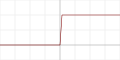
\includegraphics[scale=1]{images/Activation_binary_step.png}
\caption{Función de activación escalón binario}
\end{figure}
\item Logística / Softstep: .............. Su rango va es (0,1), y es monótona.
\begin{equation}
f(x) = \frac{1}{1+e^{-x}}
\end{equation}
\begin{figure}[htp]
\centering
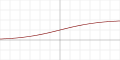
\includegraphics[scale=1]{images/Activation_logistic.png}
\caption{Funcion de activación logistica}
\end{figure}
\item Tangente hiperbólica: Esta función es utilizada por redes con salidas continuas. Un ejemplo sería el Perceptrón multicapa con retropropagación, ya que su algoritmo de aprendizaje necesita una función derivable. Cuenta con un rango (-1,1), es monótona, y se aproxima a la función identidad en su origen.
\begin{equation}
f(x) = \tanh(x) = \frac{2}{1+e^{-2x}}-1
\end{equation}
\begin{figure}[htp]
\centering
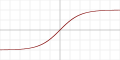
\includegraphics[scale=1]{images/Activation_tanh.png}
\caption{Funcion de activación tangencial}
\end{figure}
\item Rectificadora (ReLU - Rectified Linear Unit): Esta función de activación la introdujo por primera vez en el año 2000 Hahnloser, con motivaciones biológicas y matemáticas. Se viene usando en redes convolucionales mas que la ampliamente extendida función logística sigmoide (se basa en probabilidades), y es más practica que la tangente hiperbólica. La función rectificadora es, por tanto, una de las funciones de activación más populares para deep learning.
\begin{figure}[htp]
\centering
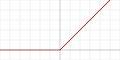
\includegraphics[scale=1]{images/Activation_rectified_linear.png}
\caption{Funcion de activación rectificadora}
\end{figure}
\item Softplus: aproximación suavizada de la funcion de activación rectificadora.
\begin{equation}
f(x) = ln(1+e^{x})
\end{equation}
\begin{figure}[htp]
\centering
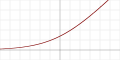
\includegraphics[scale=1]{images/Activation_softplus.png}
\caption{Funcion de activación softplus}
\end{figure}
\end{itemize}
Las propiedades deseables de una función de activación son:
\begin{itemize}
\item No lineal: Cuando contamos con una función de activación no lineal, se puede probar que una red neuronal de dos capas pueda ser una función universal de aproximación. La función identidad no satisface esta propiedad, ya que si todas las capas utilizar la funcion de activacion identidad, la red neuronal entera equivaldría a un modelo con una sola capa.
\item Continuamente diferenciable: Esta propiedad es necesaria para que sean posibles los métodos de optimización basados en el gradiente. Por ejemplo, la funcion de activación de escalón binario no es diferenciable en el 0, y su derivada es 0 en todos los demas valores, asi que los metodos basados en el gradiente no funcionan con ella.
\item Rango: Cuando el rango de la funcion de activación es finito, los métodos de entrenamiento basados en gradiente tienden a ser mas estables porque los pesos a elegir son mas limitados. Cuando el rango es infinito, el entrenamiento es por lo general mas eficiente porque los patrones afectan mas a los pesos.
\item Monotona: Cuando la funcion de activación es monotona, el error en un modelo con una sola capa tiende a converger.
\item Suavidad: Las funciones con una derivación monotona tienden a ser mas generales en algunos casos.
\item Se aproxima a la funcion identidad cerca del origen: Cuando la función de activación tiene esta propiedad, la red neuronal aprende de forma mas eficiente cuando sus pesos son inicializados con valores pequeños aleatorios.
\end{itemize}

\subsubsection {Funcion de salida}
Esta función convierte el estado de la neurona en la salida hacia la siguiente. Recordar que esta salida es transmitida mediante la sinapsis. En ocasiones podemos encontrar redes neuronales sin funcion de salida, por lo que la salida es el propio estado de activación de la neurona. Nos encontramos dos grandes tipos de funciones de salidas.
\begin{itemize}
\item Funciones de salida que transforman el estado de activación en una salida binaria. Para ello, se utiliza la función escalón.
\item Funciones de salida que transforman el estado de activacion en probabilidades. Un ejemplo de uso nos lo encontramos en la máquina de Boltzman. Las redes con etse tipo de salidas no tiene un comportamiento determinista.
\end{itemize}


\subsection{Tipos de aprendizaje en redes neuronales}
\subsubsection {Aprendizaje supervisado}
Cuando el problema nos presenta el conjunto de datos y los atributos que queremos precedir. Nos encontramos dos categorias:
\begin{itemize}
\item Regresion: los valores de salida son una o mas variables continuas. Un ejemplo sería predecir el valor de una casa en funcion de sus metros cuadrados, el numero de habitaciones, tamaño de la piscina...
\item Clasificación: los datos pertenecen a dos o mas clases, y queremos aprender como clasificar nuevas entradas en esas clases, a partir de datos que ya conocemos. Uno de los ejemplos más conocidos es el Iris dataset, donde se intenta clasificar los datos en 4 tipos de flores segun la longitud y la anchura de sus petalos y sépalos.
\end{itemize}
\subsubsection {Aprendizaje no supervisado}
Cuando no hay informacion previa de salidas dado un conjunto de entradas. En estos casos, el objetivo es encontrar grupos mediante clustering, o determinar una distribución de probabilidad sobre un conjunto de entrada.



\section {Perceptron}
En 1959, F.Rosenblatt desarrolló por primera vez la idea de Perceptrón, basandose en la regla de aprendizaje de Hebb y en los modelos de neuronas biológicas de McCulloch y Pitts. Uno de las carácteristicas que mas interés despertó de este modelo fue su capacidad para aprender a reconocer patrones.\\
El perceptron se basa en una arquitectura monocapa. Está constituido por un conjunto de celulas de entrada, que reciben los patrones a reconocer o clasificar, y una o varias celulas de salida que se ocupa de clasificar estos patrones de entrada en clases. Cada célula de entrada está conectada con todas las células de salida. En la siguiente imagen se puede observar la arquitectura de un perceptron simple con 4 entradas y 1 salida.
\begin{figure}[htp]
\centering
\vspace{-1em}
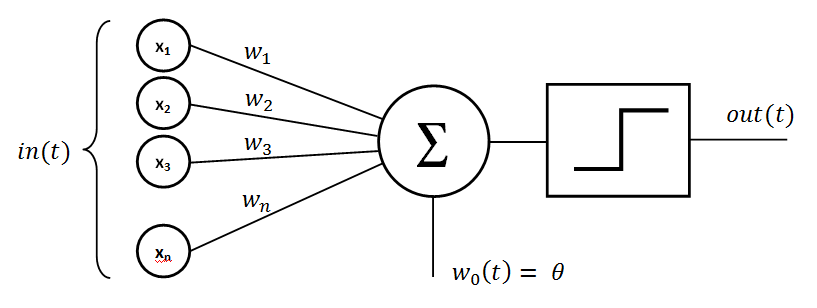
\includegraphics[scale=0.5]{images/perceptron.png}
\caption{Perceptron simple.}
\end{figure}
\\El umbral es un parámetro utilizado como factor de comparación a la hora de generar la salida. En esta arquitectura, la salida de la red se obtiene multiplicando los valores de las entradas, por los pesos de las conexiones:
\begin{equation}\label{Umbral perceptron}
y' =  \sum_{i=1}^{n} w_{i}x_{i}
\end{equation}
La salida definitiva se obtiene aplicandole la funcion de salida al nivel de activacion de la célula, es decir:
\begin{equation}\label{Salida perceptron}
y =  F(y', \theta)
\end{equation}
Con estas formulas, podemos deducir que la salida de la célula será 1 (neurona activada) si el umbral es mayor que 0, o 0 (neurona desactivada) en caso contrario.\\
La funcion de salida (F) produce una salida binaria, por lo que es un diferenciador en dos categorias. En el caso de tener unicamente dos dimensiones, la ecuación anterior se tranforma en:
\begin{equation}
w_{1}x_{1} + w_{2}x_{2} + \theta = 0
\end{equation}
Que es la ecuación de una recta con pendiente \begin{equation}-\frac{w_{1}}{w_{2}}\end{equation}, y cuyo corte en la abscina en el eje y pasa por \begin{equation}-\frac{\theta}{w_{2}}\end{equation}
Como podemos ver, podemos imaginarnos el percetron como una recta, que un gráfica de dos dimensiones, deja las dos categorías a separar a un lado y a otro de la misma.
\begin{figure}[htp]
\centering
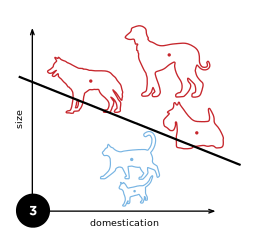
\includegraphics[scale=0.5]{images/Perceptron_example.png}
\caption{Separacion lineal del perceptrón.}
\end{figure}
\subsubsection{Aprendizaje}
El proceso de aprendizaje consiste en la inserción de un patrón de entrada del conjunto de aprendizaje perteneciente a la clase. Si la salida es correcta, no se realizará ninguna acciones, pero si no, se modificarán los pesos.
Para el perceptrón, existen 2 tipos de aprendizaje: uno utiliza una tasa de aprendizaje, mientras que el otro no la utiliza. Esta tasa de aprendizaje regula la actualización de los valores de los pesos de la red, y es la misma para todas las neuronas. Los pasos a seguir para entrenar el perceptrón son:
\begin{enumerate}
\item Inicialización de variables
\item Bucle de iteraciones:
\begin{enumerate}
\item Bucle para todos los ejemplos
\begin{enumerate}
\item Leer valores de entrada
\item Calcular error
\item Actualizar pesos segun el error
\begin{enumerate}
\item Actualizar pesos de entradas
\item Actualizarf el umbral
\end{enumerate}
\item Incremental contador de numero de ejemplos entrenados
\end{enumerate}
\item Comprobar que el vector de pesos es correcto
\item Incremental el contador de iteraciones
\end{enumerate}
\item Salida
\end{enumerate}

\subsubsection{Capacidades de un perceptrón simple}
Hasta ahora, hemos descrito el perceptrón como un clasificador. Sin embargo, tambien pueden ser usados para emular funcines lógicas elementales como AND, OR y NAND. Consideremos las funciones AND y OR. Dado que son funciones linealmente separabales, pueden ser aprendidas por un perceptrón.
\begin{figure}[htp]
\centering
\begin{minipage}[b]{0.4\textwidth}
    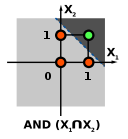
\includegraphics[scale=1]{images/perceptron_and.png}
    \caption{Separacion lineal de la funcion AND.}
  \end{minipage}
\hfill
\begin{minipage}[b]{0.4\textwidth}
    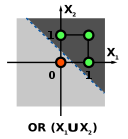
\includegraphics[scale=1]{images/perceptron_or.png}
  \caption{Separacion lineal de la funcion OR.}
  \end{minipage}
\end{figure}
\\Sin embargo, la función XOR no puede ser aprendida por un unico perceptrón, ya que requerie el uso de al menos del lineas para separar las clases. Si se quiere alcanzar esta funcionalidad, es necesario utilizarse al menos una capa mas. Aquí es donde entra en juego el perceptrón multicapa.

\section {Perceptron multicapa}
El perceptrón muticapa tuvo su origen en los años 80, con la idea de solucionar el mayor problema del perceptron simple: no ser capaz de aprender funciones no linealmente separables (como es el caso de la función XOR). Se ha demostrado que es un aproximador universal de funciones.
\\El perceptrón multicapa es un modelo de red neuronal con alimentacion hacia delante, es decir, con conexiones sin bucles (tipo de red feedforward). Está compuesto de varias capas ocultas entre la entrada y la salida de la misma, y caracterizado por tener salidas disjuntas pero relacionadas entre si, ya que la salida de una neurona es la entrada de la siguiente.
\begin{figure}[htp]
\centering
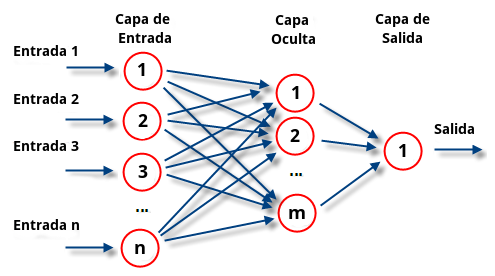
\includegraphics[scale=1.2]{images/multilayerperceptron.png}
\caption{Perceptrón multicapa.}
\end{figure}
\\Las capacidades de decisión de un perceptron multicapa de 2 y 3 capas con una unica neurona de salida se muestran en la siguiente tabla:
\begin{figure}[htp]
\centering
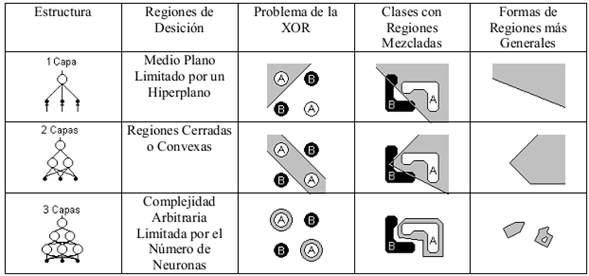
\includegraphics[scale=0.7]{images/perceptron23capas.png}
\end{figure}
\\En el perceptrón multicapa, al igual que en el perceptrón simple, podemos diferenciar una fase de propagación de los valores de entrada hacia delante, y una fase de aprendizaje en la que los datos obtenidos a la salida del perceptrón se van propagando hacia atrás para observar el error y actualizar los pesos de las neuronas. Este algorirmo se llama backpropagation o retropropagación.
\subsection{Propagación}
Imaginemos un perceptrón multicapa con C capas. Llamemos ${W^{C} = W^{c}_{ij}}$ a la matriz de pesos de la capa c y c+1, donde ${W^{c}_{ij}}$ representa el peso de la neurona i de la capa c a la neurona j de la capa c+1. Denominaremos ${U^{C} = u^{c}_{i}}$ al vector de umbrales de las neuronas de la capa c. Se denomina ${a^{c}_{i}}$ a la activación o entrada de la neurona i de la capa c. Las activaciones de las neuronas se calculan de forma distinta dependiendo de la capa en la que nos encontremos.
\begin{itemize}
\item Capa de entrada: la activación se corresponde con el patrón de entrada del perceptrón.
\item Capa oculta: la activación procede de las salidas de las capas anteriores conectadas a las neuronas de esta capa. Esta activación se calcula como la suma de los productos de las activaciones que reciben las neuronas de las capas anteriores multiplicadas por su peso, añadiendoles el umbral, es decir:\\
\begin{equation}
a_{i}^{c} = f(\sum_{j=1}^{n_{c-1}}w_{ji}^{c-1}a_{j}^{c-1}+u_{i}^{c})
\end{equation}
\item Capa de salida: ocurre lo mismo que en las capas ocultas, salvo que ahora la salida de las neuronas se corresponde con la salida de la red.
\end{itemize}
La funcion f es a lo que llamamos funcion de activación. Las funciones de activación mas utilizadas en el perceptrón multicapa son la función sigmoidal y la función tangente hiperbólica. Ambas poseen un intervalo continuo dentro de [0,1] y [-1,1] y vienen dadas por las siguientes ecuaciones.
\begin{itemize}
\item Función sigmoidal ${f_{sigm}(x)=\frac{1}{1+e^{-x}}}$
\item Función tangente hiperbólica ${f_{thip}(x)=\frac{1-e^{-x}}{1+e^{-x}}}$
\end{itemize}
\begin{figure}[htp]
\centering
\vspace{-1.5em}
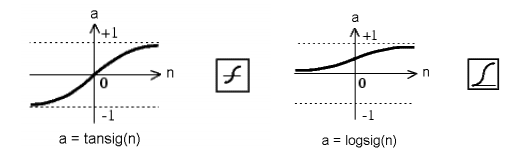
\includegraphics[scale=0.6]{images/tansig_vs_logsig.png}
\end{figure}
Ambas funciones estan relacionadas mediante la expresión ${f_{thip}(x)=2f_{sigm}(x)-1}$, por lo que la utilización de una u otra depende de cual sea mas compatible con el tipo de patrón que se va a utilizar. La funcion sigmoidal tiene un nivel de saturación inferior igual a 0, y la tangente hiperbólica lo tiene a -1.\\
Normalmente, la función de activacion suele ser la misma para todas las neuronas de la red exceptuando las neuronas de la capa de salida, que suelen utilizar dos funciones distintas: la funcion identidad, y la función escalon.
\subsection{Consideraciones de diseño}
A la hora de diseñar un perceptrón multicapa para abordar un problema, el primer paso es determinar la arquitectura de la red. Esto implica determinar tres variables, ya explicadas anteriormente:
\begin{itemize}
\item Función de activación: se elige según el recorrido deseado, pero no influye en la capacidad de la red para resolver el problema.
\item Numero de neuronas de entrada y de salida: viene dado por la definicion del problema. En ocasiones esta afirmación no tiene porque ser del todo cierta, y se ha de proceder a hacer un analisis previo basandose en tecnicas de analisis de correlacion, de sensebilidad, de importancia relativa...
\item Numero de capas ocultas: pese a ser una variable que ha de definir el diseñador, no existe un mé'todo que determine el numero óptimo de neuronas ocultas para resolver el problema. Partiendo de una arquitectura ya entrenada, se van realizando pequeños cambios en el numero de neuronas/capas ocultas para buscar así el diseño optimo, ya que existen muchos tipos de arquitectura capaces de resolver un mismo problema.
\end{itemize}
\subsection{Algoritmo de Retropropagacion o Backpropagation}
Como se ha comentado anteriormente, el proceso de aprendizaje del perceptron multicapa consiste en propagar hacia atrás cierta informacion desde la salida del perceptrón hasta su entrada. Esta información será el error entre la salida obtenida y la salida esperada, con el objetivo de que en las siguientes iteraciones la salida obtenida se aproxime lo máximo prosible a la salida esperada. Por tanto, nos encontramos ante un algoritmo de aprendizaje supervisado.\\
Hay muchos errores que se pueden utilizar, pero el perceptrón multicapa usa la función error cuadrático medio, que se define como:
\begin{equation}
e(n) = \frac{1}{2}\sum_{i=1}^{n_{c}}(s_{i}(n)-y_{i}(n))^{2}
\end{equation}
siendo n cada una de las iteraciones del aprendizaje. El error obtenido e(n) es el error de una sola iteracion, por lo que si queremos entrenar la red con varios patrones, el error medio de esta será ${E=\frac{1}{N}\sum_{n=1}^{N}e(n)}$. En resumen, el perceptrón multicapa aprende encontrando el minimo de la función de error.\\
Aunque el aprendizaje debe llevarse a cabo minimizando el error total, los metodos más utilizados son los basados en metodos de gradiente estocástico, que consisten en minimizar el error en cada patron e(n). Por tanto, aplicando el metodo de gradiente descendiente, cada peso de la red w se actualiza para cada patrón de entrada n, y siendo ${\alpha}$ la tasa de aprendizaje, de acuerdo con la siguiente ecuacion:
\begin{equation}
w(n)=w(n-1)-\alpha \frac{\partial e(n)}{\partial w}
\end{equation}
Dado que las neuronas de la red están agrupadas en capas ocultas segun niveles, es posible aplicar el metodo del gradiente descendente de forma eficiente en todas las neuronas, llevando a cabo el algoritmo de retropropagacion o regla delta generalizada.

\subsection{Regla delta generalizada}
Como ya se ha comentado, la regla delta generalizada no es mas que una forma eficiente de aplicar el método de gradiente a los parametros de la arquitectura (pesos y umbrales). Su aprendizaje es supervisado. Su uso consiste en ajustar pesos y bias tratando de minimizar la suma del error cuadrático. Para ello, se cambian dichas variables en la dirección contraria a la pendiente del error.\\
Las redes neuronales entrenadas mediante esta técnica, dan respuestas mas que razonables cuando al sistema se le presentan entradas que nunca habia analizado. A una nueva entrada, le hará corresponder una entrada similar a la salida obtenida para un patrón de entrenamiento, siendo éste similar al patrón presentado a la red. Esta es una de las grandes propiedades de la regla delta, su capacidad de generalicación.\\
Podriamos describir su funcionamiento básico en una serie de pasos:
\begin{itemize}
\item Se introduce un vector de entrada, y se calcula su salida.
\item Se calcula el error
\item Se determina en que direccion se deben cambiar los pesos para minimizar el error
\item Se determina la cantidad en la que se cambiará cada peso
\item Se modifican los pesos.
\item Se repiten los pasos del 1 al 5 con todos los patrones de entrenamiento, hasta que el error de los vectores sea lo más reducido posible.
\end{itemize}

\subsection{Tasa de aprendizaje}
La tasa de aprendizaje (${\alpha}$) es un parámetro que determina la velocidad a la que van a cambiar los pesos de las conexiones de la red. Tiene un rango [0,1], siendo los valores mas cercanos a cero los que hacen que los pesos cambien poco a poco, acercandose lentamente a la convergencia, y los cercanos a uno los que hacen que la red converja mas rapidamente al principio, pero siendo posible que los pesos oscilen demasiado al encontrar el peso óptimo final. Por esta razón es importante encontrar una tasa de aprendizaje óptima.\\
Aquí es donde entra en juego un segundo termino llamado momento (${\eta}$), que pondera cuanto queremos que influya lo que los pesos han cambiado en la anterior iteración. Con ello, sabremos que si los pesos han cambiado mucho, es que estamos aun lejos del valor de la tasa de aprendizaje óptimo, por lo que avanzaremos en su busqueda mas rapidamente. Por otro lado, si los pesos no han cambiado a penas, sabremos que el valor optimo de ${\alpha}$ está cerca.\\
Podemos modificar la ecuacion 2.XXXXXXXX para añadir esta mejora, de la siguiente manera:
\begin{equation}
w(n) = w(n-1) = - \alpha \frac{\partial e(n)}{\partial w} + \eta \Delta w(n-1)
\end{equation}
siendo ${\Delta}$w(n-1)=w(n-1)-w(n-2) el incremento que sufrió el parametro w en la anterior iteración.
\subsection{Sobreajuste y early stopping}
El sobreajuste o overfitting es el efecto secundario de sobreentrenar un algoritmo de aprendizaje con ciertos datos para los que ya se conoce el resultado deseado. El algortismo debe alcanzar un estado en el cual sea capaz de predecir otros casos a partir de lo ya aprendido mediante datos de entrenamiento, generalizando para poder resolver distintas situaciones a las ya presentes durante el entrenamiento. No obstante, cuando un sistema se entrena demasiado o se entrena con datos extraños, el algoritmo tiende a quedarse ajustado a unas caracteristicas muy especificas de los datos de entrenamiento, que no representan un estado general de problema. En este estado, nuestro diseño es mas eficaz al responder a muestras del conjunto de entrenamiento, pero ante nuevas entradas el resultado empeora.\\
Una manera de resolver este problema es extraer un conjunto de entradas del dataset de entrenamiento, y utilizarlo de manera auxiliar a modo de validación. Ya que este subconjunto se deja al margen durante el entrenamiento, su objetivo será evaluar el error en la red tras cada epoch, para determinar cuando este empieza a aumentar. Cuando aumente, se prodecerá a detener el entrenamiento y se conservarán los valores de los pesos del ciclo anterior. A este método se le llama early-stopping.

\section{Redes neuronales convolucionales}
Las redes neuronales convolucionales son muy similares a las redes neuronales ordinarias descritas hasta ahora, como el perceptrón multicapa. Las neuronas tienen pesos, sesgos, reciben una entrada con la que realiza un producto escalar y sobre la que aplica una función de activación, tienen una función de perdida...\\
Sin embargo, se utilizan principalmente para resolver el mayor problema que tienen las redes neuronales ordinarias: el tratamiento de imágenes. Pese a que con las redes neuronales estándar es posible manejar imágenes (veremos el ejemplo del MNIST en el apartado 4.3), en cuanto las imágenes aumentan su tamaño y calidad esto se vuelve intratable. Al tratarse de neuronas totalmente conectadas, provocaríamos un desperdicio de recursos así como un rápido sobreajuste.\\
Las redes neuronales convolucionales trabajan dividiendo y modelando la información en partes mas pequeñas, y combinando esta información en las capas mas profundas de la red. Por ejemplo, en el caso del tratamiento de una imagen, las primeras capas tratarían de detectar los bordes de las figuras. Las siguientes capas buscarían combinar los patrones de detección de bordes para conseguir formas mas simples, y aplicar patrones de posición de objetos, iluminación... Por ultimo, en las últimas capas se intentará hacer coincidir la imagen con todos los patrones descubiertos, para conseguir una predicción final de la suma de todos ellos. Así es como las redes neuronales convolucionales consiguen modelar una gran cantidad de datos, dividiendo previamente el problema en partes para conseguir predicciones mas sencillas y precisas.
\subsection{Estructura}
En general, todas las redes neuronales convoluciones están formadas por una estructura compuesta por 3 tipos de capas:
\subsubsection{Capa convolucional}
Esta capa le da nombre de la red. En vez de utilizar la multiplicación de matrices como en la redes neuronales estándar, se aplica una operación llamada convolución. Esta operación recibe como entrada una imagen, y sobre ella aplica un filtro que nos devuelve su mapa de características, reduciendo así el tamaño de sus parámetros. La convolución utiliza tres ideas que ayudan a mejorar cualquier sistema sobre el que se aplique machine learning:
\begin{itemize}
\item{\textbf{Iteracciones dispersas}:}
Al aplicar un filtro de menos tamaño sobre la entrada, reducimos bastante el numero de parámetros y cálculos.
\item{\textbf{Parametros compartidos}:}
Compartir parámetros entre los distintos tipos de filtros ayuda a mejorar la eficiencia del sistema.
\item{\textbf{Representaciones equivariantes}:}
Si las entradas cambian, las salidas cambian de forma similar.
\end{itemize}
Además, la convolución proporciona herramientas para trabajar con entradas de tamaño variable, lo cual es muy útil cuando se trabaja con imágenes (cada imagen tiene un numero distinto de píxeles). Se basa en un operador matemático que transforma dos funciones f y g, en una tercera, que en cierto sentido, representa la magnitud en la que se superponen f y una versión trasladada y rotada de g.
\begin{figure}[htp]
\centering
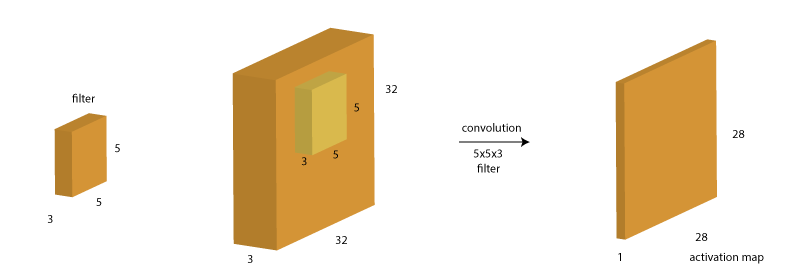
\includegraphics[scale=0.7]{images/conv_layer.png}
\caption{Funcionamiento de capa convolucional}
\end{figure}\\
\subsubsection{Capa de reducción o pooling}
Esta capa se coloca generalmente después de la capa convolucional. Es la encargada de reducir la cantidad de parámetros a analizar reduciendo las dimensiones espaciales (ancho x alto), quedándose de esta forma con las características mas comunes. La operación que lleva a cabo esta capa también se llama reducción de muestreo, ya que la reducción de tamaño implica también una perdida de información. Sin embargo, para un red neuronal, este tipo de pérdida puede ser beneficioso debido a:
\begin{itemize}
\item La reducción del tamaño provoca una menor sobrecarga de calculo en las próximas capas de la red.
\item Reduce habitualmente el sobreajuste.
\end{itemize}
La operación que se suele aplicar en esta capa es "max-pooling", que divide la imagen de entrada en un conjunto de rectángulos, y respecto a cada uno de ellos, se queda con el valor máximo.
\begin{figure}[htp]
\centering
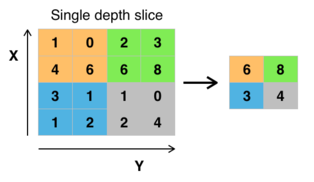
\includegraphics[scale=0.7]{images/max_pooling.png}
\caption{Max-pooling aplicado a una imagen}
\end{figure}
\subsubsection{Capa clasificadora totalmente conectada}
Una vez que la imagen ha pasado tanto por las capas convolucionales como las de pooling y se han extraído sus características mas destacadas, los datos llegan a la fase de clasificación. Para ello, ĺas redes convolucionales normalmente utilizan capas completamente conectadas en las que cada píxel se trata como una neurona independiente. Las neuronas de esta fase funcionan como las de un perceptrón multicapa, donde la salida de cada neurona se calcula multiplicando la salida de la capa anterior por el peso de la conexión, y aplicando a este dato una función de activación.

\section{Redes neuronales recurrentes}
Los humanos no empiezan a pensar de cero a cada segundo. Por ejemplo, mientras leemos, entendemos cada palabra basándonos en el contexto que forman las palabras previas. No desperdiciamos los ideas anteriores, sino que estas tienen persistencia en la memoria.\\
Las redes neuronales tradicionales no cuentan con esta capacidad, y es su mayor defecto. Por ejemplo, imaginemos el caso en el que queremos clasificar que clase de evento está pasando en una punto de una película. No está muy claro cómo una red neuronal tradicional podría usar razonablemente las escenas anteriores para predecir las siguientes.\\
Y aquí es donde entran en juego las redes neuronales recurrentes, ya que estas sí resuelven este problema. Su principal característica es que son redes con bucles, que permiten que la información persista.\\
\begin{figure}[htp]
\centering
\vspace{-1.5em}
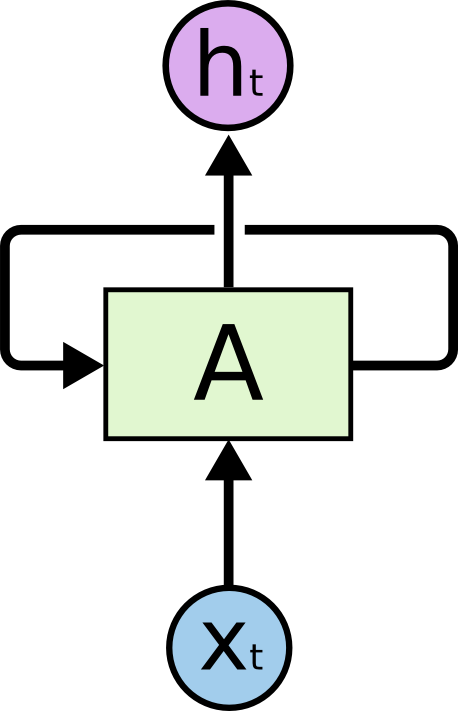
\includegraphics[scale=0.3]{images/rnnrolled.png}
\caption{Ejemplo básico de red neuronal recurrente.}
\end{figure}
\\En el diagrama 2.18, podemos ver como una parte de la red neuronal, \textbf{A}, recibe una entrada \textbf{x} y devuelve una salida \textbf{h}. El bucle permite que la información pase de un ciclo de la red al siguiente. Pese a que el concepto de bucle parezca algo extraño, las redes neuronales que cuentan con ellos no son tan distantes de la redes neuronales tradicionales. Una red neuronal recurrente puede ser creada utilizando múltiples copias de la misma red, pasando el mensaje o salida al nodo sucesor. Si desenrollamos el bucle, tendríamos algo parecido a la figura 2.19:\\
\begin{figure}[htp]
\centering
\vspace{-1.5em}
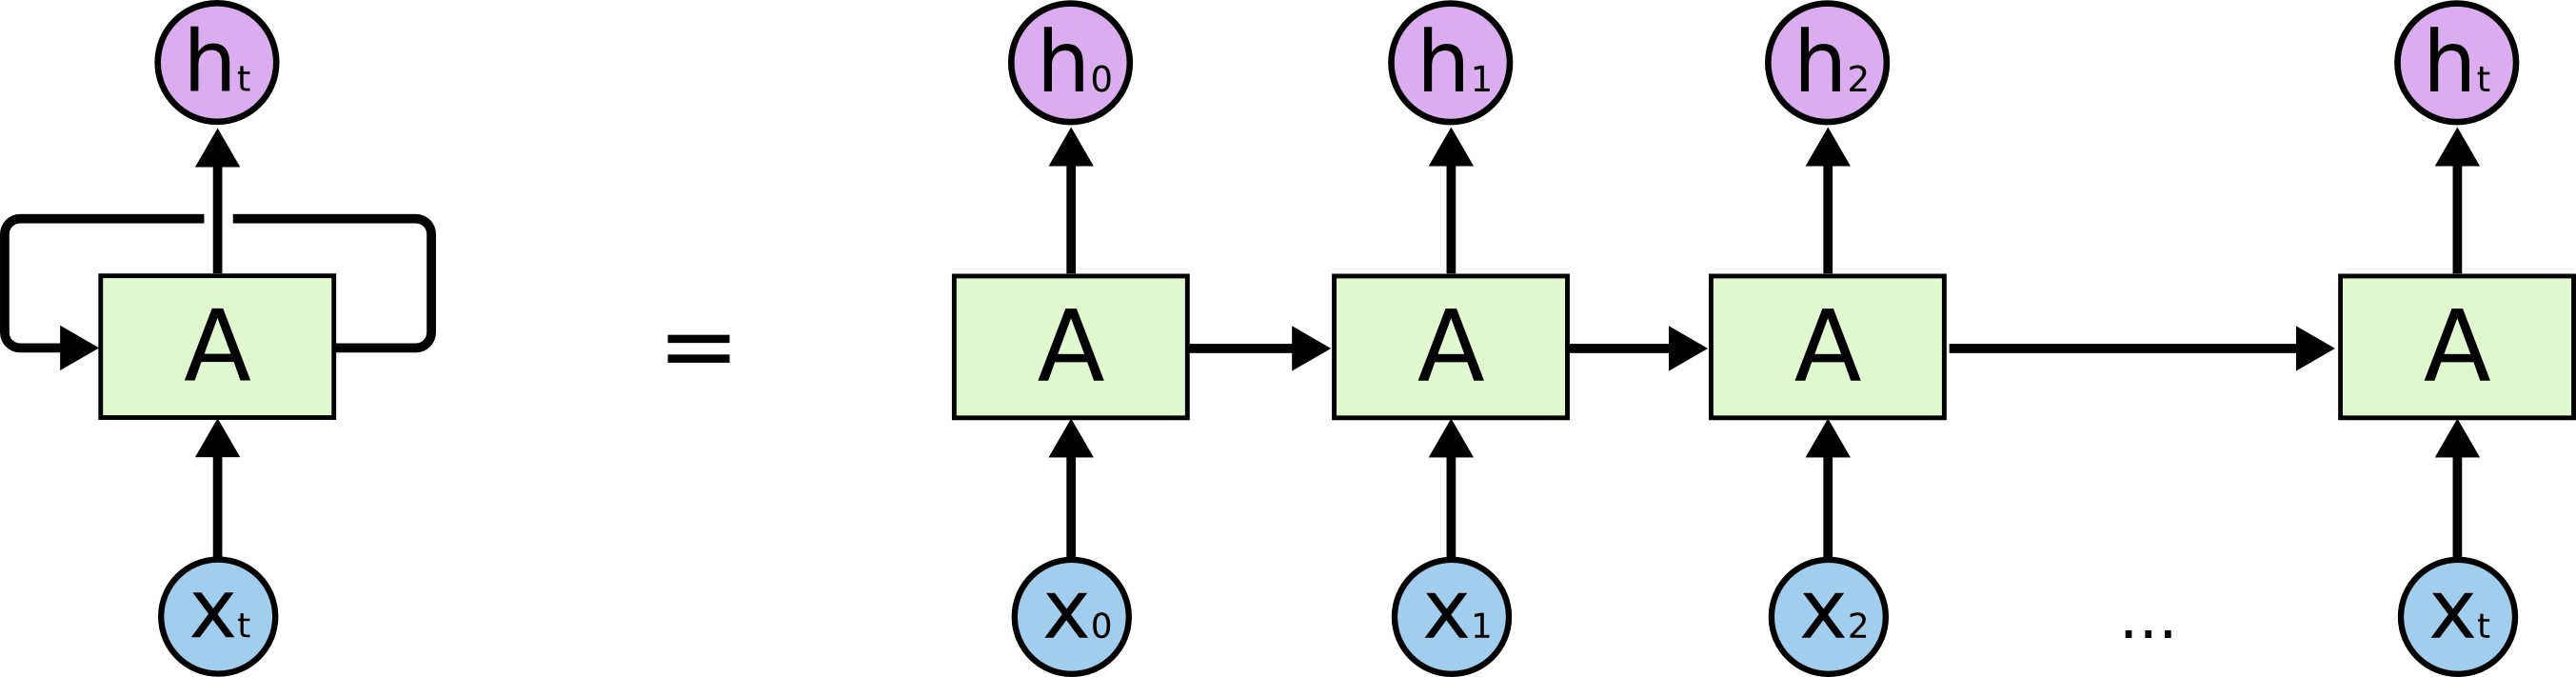
\includegraphics[scale=0.3]{images/RNNunrolled.png}
\caption{Red neuronal recurrente desenrollada.}
\end{figure}
\\Esta forma de cadena hace prever que las redes neuronales recurrentes están íntimamente relacionadas con secuencias y listas. En los últimos años, se han logrado auténticos grandes éxitos aplicando las RNN para resolver problemas como: reconocimiento de discursos, modelación de lenguajes, traducciones, captación de imágenes... Un factor clave en estos éxitos es el uso de las redes LSTMs, un tipo muy especial de redes neuronales recurrentes que trabajan por muchas razones de forma mas eficiente que la versión estándar.
\subsubsection{El problema de la longitud de las dependencias.}
Uno de los intereses de las RNNs es la idea de conectar información antigua con la tarea actual. En temas de vídeo, sería útil por ejemplo utilizar frames anteriores para entender el frame actual, pero... ¿pueden las RNN hacer esto? La respuesta es, depende.\\
Algunas veces, solo necesitamos utilizar información reciente para la tarea actual. Por ejemplo, en temas de modelación de lenguaje, para adivinar la siguiente palabra en un contexto, en la mayoría de los casos bastaría con analizar la frase en la que se encuentra. Sin embargo, hay casos en los que se necesita acceder a un contexto mas grande. Desafortunadamente, a medida que el espacio entre la información requerida y la tarea actual aumenta, las RNN tardan cada vez más en aprender a conectar la información.\\
\begin{figure}[htp]
\centering
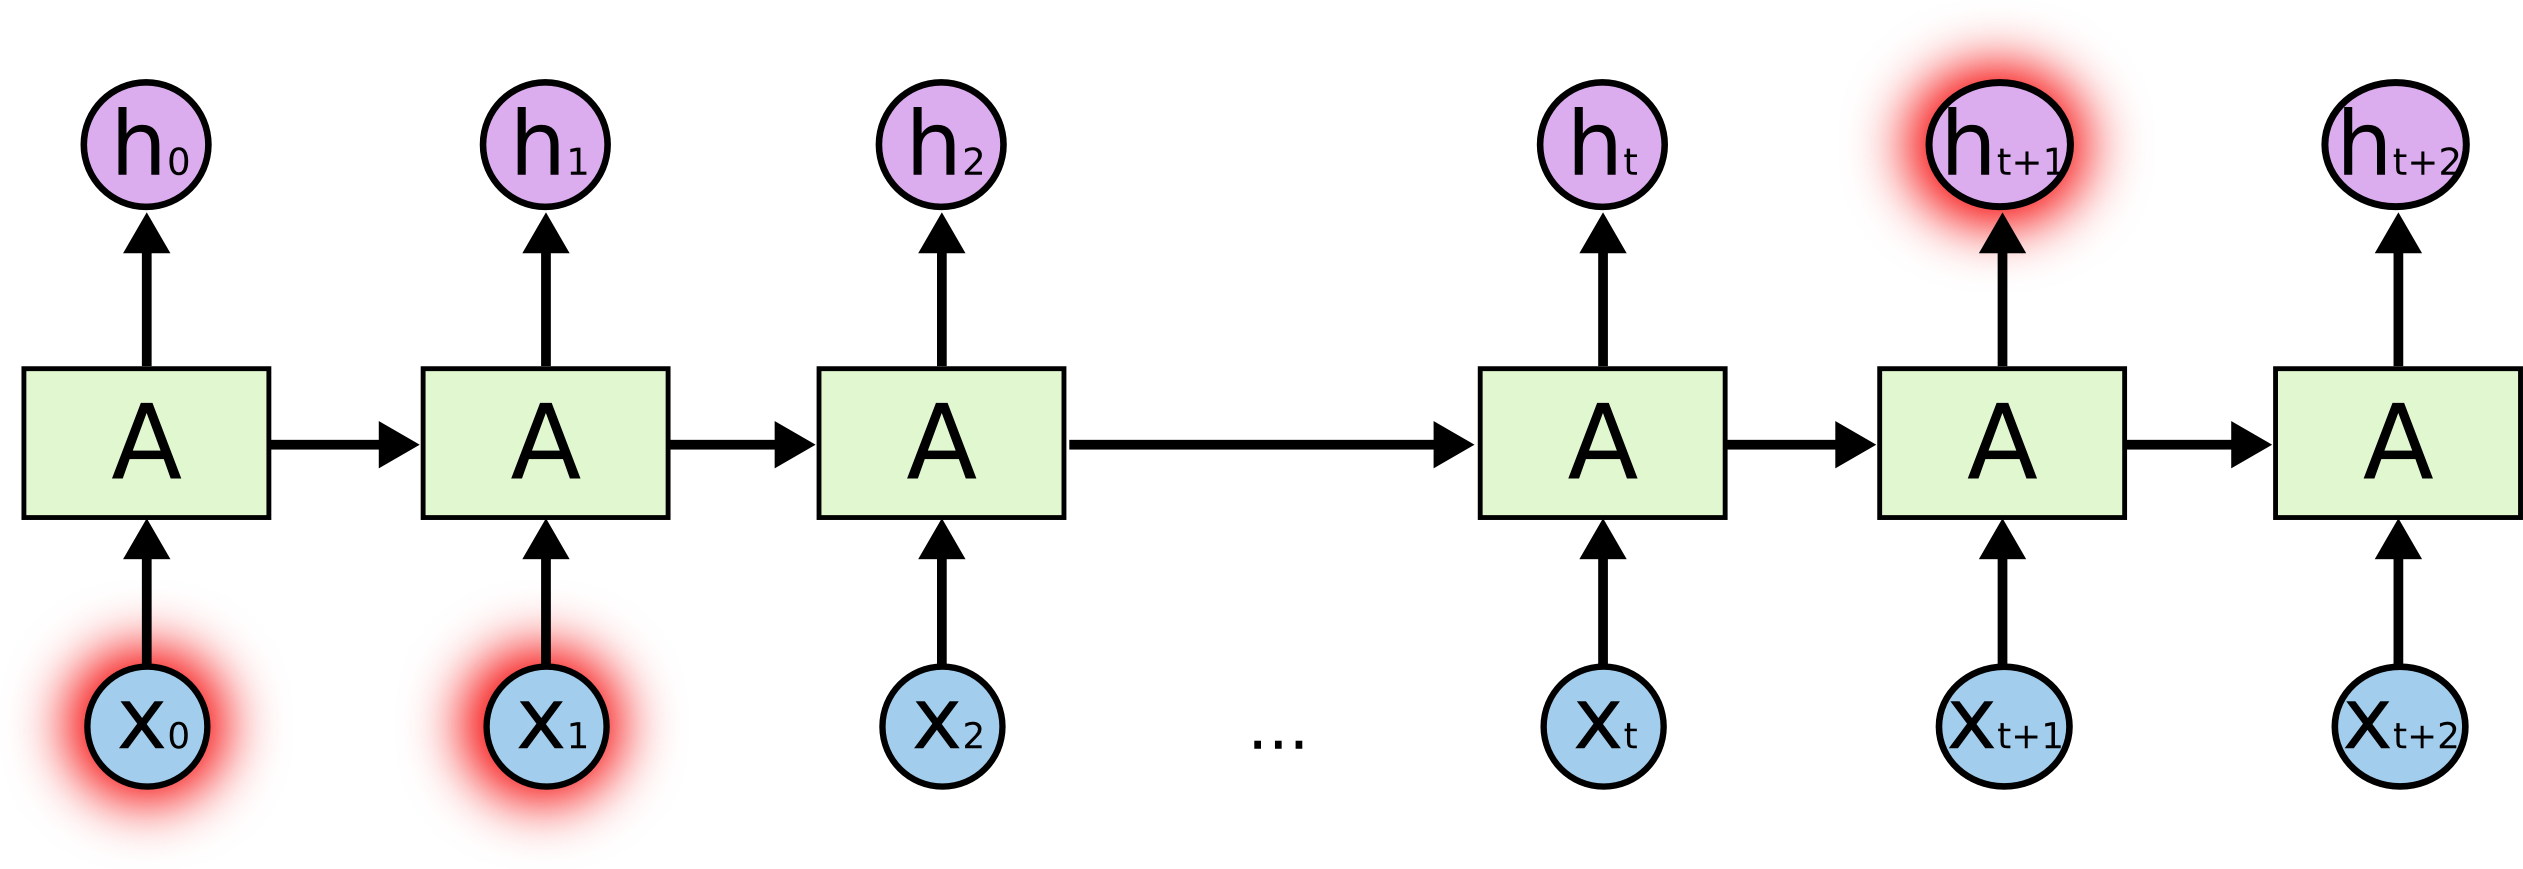
\includegraphics[scale=0.3]{images/RNN-longtermdependencies.png}
\caption{Red neuronal recurrente desenrollada.}
\end{figure}
\\En teoría, las RNN son perfectamente capaces de resolver este problema (long-term dependencies), pero en la práctica no lo parece tanto. En 1991, Hochreiter estudió este problema, y encontró algunas razones por las que las RNN encuentran dificultades a la hora de aprender información sobre grandes contextos. Por suerte, las redes LSTMs solventan estos problemas.
\subsection{Redes LSTM}
Las redes Long Short Term Memory (normalmente llamadas LSTMs) son un tipo especial de redes neuronales recurrentes descritas por primera vez en 1997 por Hochreiter \& Schmidhuber, capaces de aprender una larga lista de dependencias en largos periodos de tiempo.\\
Todas las redes neuronales recurrentes tienen forma de cadena al repetir sus módulos. En las RNN estándar, el modulo repetidor tiene una estructura muy simple, con una sola capa, como podría ser la de tipo tanh. Las redes LSTM tambien tienen forma de cadena, pero el modulo repetidor en vez de tener una sola capa, tiene cuatro.
\begin{figure}[htp]
\centering
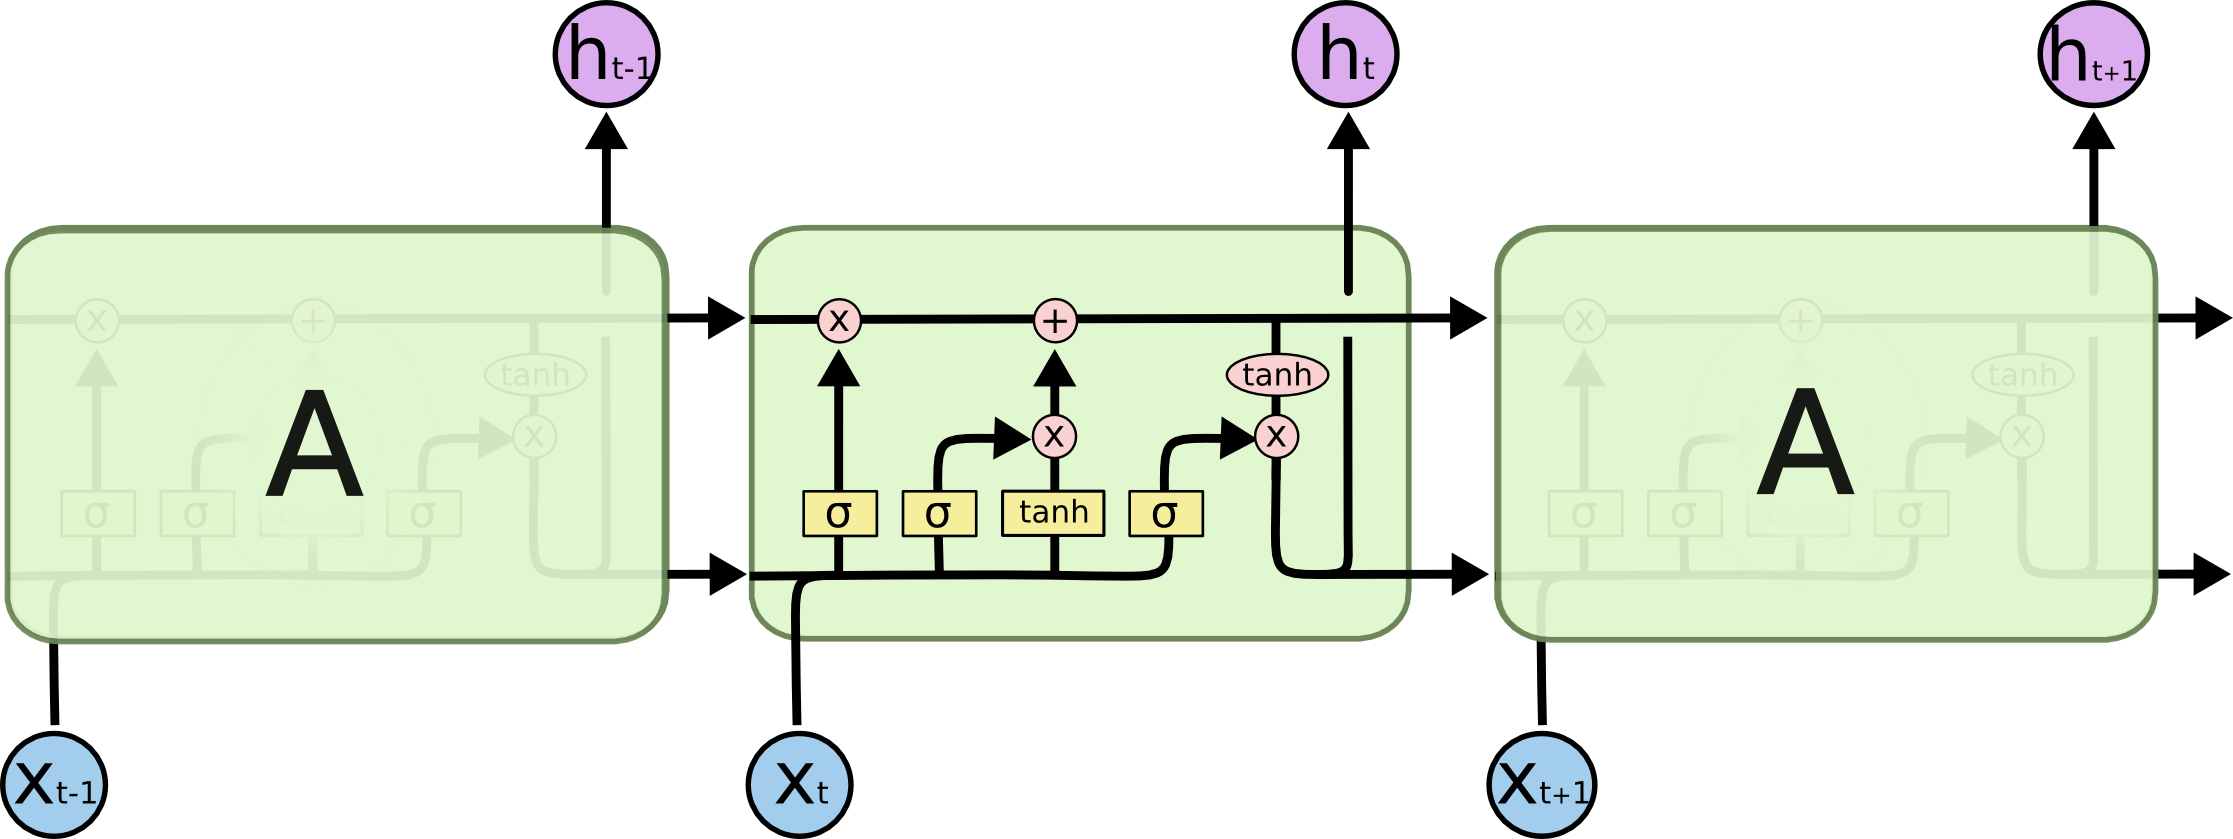
\includegraphics[scale=0.35]{images/LSTM3-chain.png}
\caption{Estructura del modulo repetidor.}
\end{figure}
\begin{figure}[htp]
\centering
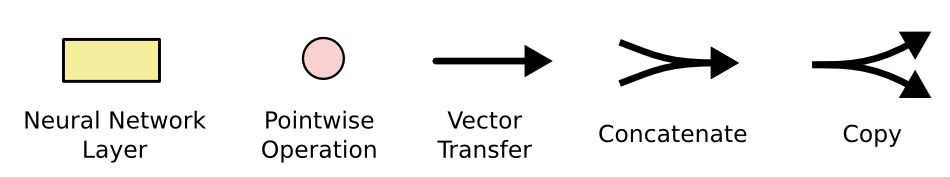
\includegraphics[scale=0.2]{images/LSTM2-notation.png}
\caption{Notación del modulo repetidor.}
\end{figure}
\\La clave de las redes LSTMs se encuentra en el estado de la celda, es decir, en la linea horizontal que recorre la parte superior del diagrama 2.21, ya que permite a la información fluir por toda la red con solo algunas pequeñas interacciones, sin ser a penas alterada.
La red también tiene la habilidad de borrar o añadir información al estado de la celda mediante estructuras llamadas puertas. Estas puertas son una manera de permitir opcionalmente a la información circular o no, y se componen de una capa sigmoide y una operación de multiplicación. Las salidas de la capa sigmoide alternan entre 0 y 1, describiendo si la información fluye o no. Una red LSTM tiene 3 de estas puertas, para proteger y controlar el estado de la celda.\\\\
Las redes neuronales LSTM siguen una serie de pasos para decidir qué información se va a ir almacenando o borrando. Podemos destacar los siguientes:
\begin{enumerate}
\item \textbf{Decidir qué información despreciar}. Esta decisión la toma la capa sigmoide, que devuelve una salida igual a 1 si se busca mantener la información, o 0 si queremos deshacernos de ella.\\
Volvamos al ejemplo de modelado del lenguaje, donde se quiere predecir una palabra basándose en las anteriores. En este problema, el estado de la celda puede almacenar el género del sujeto para usar los pronombres adecuados. Cuando nos encontremos un nuevo sujeto, olvidaremos el genero del anterior ya que no será de utilidad.
\item \textbf{Decidir que información se va a almacenar}. Consta de dos partes: primero, una capa sigmoide decide que valores son actualizados. Después, una capa tanh crea un vector con los nuevos valores candidatos, que pueden ser añadidos al estado.\\
En el ejemplo anterior, se decidiría que queremos añadir el género del nuevo sujeto al estado de la celda, para reemplazar el viejo que queremos olvidar.
\item \textbf{Actualizar el estado de la celda}. En el paso anterior se decide que hacer, y ahora toca hacerlo. Se multiplica el viejo estado por la salida de la capa sigmoide del primer paso, olvidando así las cosas que decidimos olvidar. A esto, se le suma el producto de la salida de la capa sigmoide y de la capa tanh del segundo paso. Con ello, se consiguen saber los nuevos valores candidatos, escalados según la decisión de actualizar el estado de la celda.\\
En el caso de modelado de lenguaje, ahora es cuando se desecha la información sobre el género del viejo sujeto, y se añade la nueva información, como decidimos en los pasos anteriores.
\item \textbf{Decidir la salida basandonos en el estado de la celda, pero de manera filtrada}. Primero, mediante una capa sigmoide, se decide que partes del nuevo estado de la celda se van a sacar como salida. Después, se pasa el estado de la celda por una capa tanh para tener valores entre -1 y 1, y lo multiplicamos por la salida de la capa sigmoide, para sacar solo las partes que decidamos.\\
En el ejemplo de modelado de lenguaje, una vez que se encuentre el nuevo sujeto, se sacará información a cerca de él como puede ser si éste es singular o plural, para después poder conjugar correctamente el verbo que le sigue.
\end{enumerate}
Como se ha comentado anteriormente, la mayoría de los mejores resultados utilizando redes recurrentes, es mediante las redes LSTMs. Pero a pesar de que su descubrimiento ha sido un gran hito, todavía quedan metas por cumplir. Una de ellas sería dotar a las RNN de una capacidad para decidir que información consultar en una fuente muy grande de información. Por ejemplo, si estamos usando redes RNN para crear un titulo que describa una imagen, sería útil elegir que partes de la imagen usar para cada palabra.
\label{ch:teoria}
